% Options for packages loaded elsewhere
\PassOptionsToPackage{unicode}{hyperref}
\PassOptionsToPackage{hyphens}{url}
\PassOptionsToPackage{dvipsnames,svgnames,x11names}{xcolor}
%
\documentclass[
  letterpaper,
  DIV=11,
  numbers=noendperiod]{scrreprt}

\usepackage{amsmath,amssymb}
\usepackage{iftex}
\ifPDFTeX
  \usepackage[T1]{fontenc}
  \usepackage[utf8]{inputenc}
  \usepackage{textcomp} % provide euro and other symbols
\else % if luatex or xetex
  \usepackage{unicode-math}
  \defaultfontfeatures{Scale=MatchLowercase}
  \defaultfontfeatures[\rmfamily]{Ligatures=TeX,Scale=1}
\fi
\usepackage{lmodern}
\ifPDFTeX\else  
    % xetex/luatex font selection
\fi
% Use upquote if available, for straight quotes in verbatim environments
\IfFileExists{upquote.sty}{\usepackage{upquote}}{}
\IfFileExists{microtype.sty}{% use microtype if available
  \usepackage[]{microtype}
  \UseMicrotypeSet[protrusion]{basicmath} % disable protrusion for tt fonts
}{}
\makeatletter
\@ifundefined{KOMAClassName}{% if non-KOMA class
  \IfFileExists{parskip.sty}{%
    \usepackage{parskip}
  }{% else
    \setlength{\parindent}{0pt}
    \setlength{\parskip}{6pt plus 2pt minus 1pt}}
}{% if KOMA class
  \KOMAoptions{parskip=half}}
\makeatother
\usepackage{xcolor}
\setlength{\emergencystretch}{3em} % prevent overfull lines
\setcounter{secnumdepth}{5}
% Make \paragraph and \subparagraph free-standing
\makeatletter
\ifx\paragraph\undefined\else
  \let\oldparagraph\paragraph
  \renewcommand{\paragraph}{
    \@ifstar
      \xxxParagraphStar
      \xxxParagraphNoStar
  }
  \newcommand{\xxxParagraphStar}[1]{\oldparagraph*{#1}\mbox{}}
  \newcommand{\xxxParagraphNoStar}[1]{\oldparagraph{#1}\mbox{}}
\fi
\ifx\subparagraph\undefined\else
  \let\oldsubparagraph\subparagraph
  \renewcommand{\subparagraph}{
    \@ifstar
      \xxxSubParagraphStar
      \xxxSubParagraphNoStar
  }
  \newcommand{\xxxSubParagraphStar}[1]{\oldsubparagraph*{#1}\mbox{}}
  \newcommand{\xxxSubParagraphNoStar}[1]{\oldsubparagraph{#1}\mbox{}}
\fi
\makeatother


\providecommand{\tightlist}{%
  \setlength{\itemsep}{0pt}\setlength{\parskip}{0pt}}\usepackage{longtable,booktabs,array}
\usepackage{calc} % for calculating minipage widths
% Correct order of tables after \paragraph or \subparagraph
\usepackage{etoolbox}
\makeatletter
\patchcmd\longtable{\par}{\if@noskipsec\mbox{}\fi\par}{}{}
\makeatother
% Allow footnotes in longtable head/foot
\IfFileExists{footnotehyper.sty}{\usepackage{footnotehyper}}{\usepackage{footnote}}
\makesavenoteenv{longtable}
\usepackage{graphicx}
\makeatletter
\newsavebox\pandoc@box
\newcommand*\pandocbounded[1]{% scales image to fit in text height/width
  \sbox\pandoc@box{#1}%
  \Gscale@div\@tempa{\textheight}{\dimexpr\ht\pandoc@box+\dp\pandoc@box\relax}%
  \Gscale@div\@tempb{\linewidth}{\wd\pandoc@box}%
  \ifdim\@tempb\p@<\@tempa\p@\let\@tempa\@tempb\fi% select the smaller of both
  \ifdim\@tempa\p@<\p@\scalebox{\@tempa}{\usebox\pandoc@box}%
  \else\usebox{\pandoc@box}%
  \fi%
}
% Set default figure placement to htbp
\def\fps@figure{htbp}
\makeatother
% definitions for citeproc citations
\NewDocumentCommand\citeproctext{}{}
\NewDocumentCommand\citeproc{mm}{%
  \begingroup\def\citeproctext{#2}\cite{#1}\endgroup}
\makeatletter
 % allow citations to break across lines
 \let\@cite@ofmt\@firstofone
 % avoid brackets around text for \cite:
 \def\@biblabel#1{}
 \def\@cite#1#2{{#1\if@tempswa , #2\fi}}
\makeatother
\newlength{\cslhangindent}
\setlength{\cslhangindent}{1.5em}
\newlength{\csllabelwidth}
\setlength{\csllabelwidth}{3em}
\newenvironment{CSLReferences}[2] % #1 hanging-indent, #2 entry-spacing
 {\begin{list}{}{%
  \setlength{\itemindent}{0pt}
  \setlength{\leftmargin}{0pt}
  \setlength{\parsep}{0pt}
  % turn on hanging indent if param 1 is 1
  \ifodd #1
   \setlength{\leftmargin}{\cslhangindent}
   \setlength{\itemindent}{-1\cslhangindent}
  \fi
  % set entry spacing
  \setlength{\itemsep}{#2\baselineskip}}}
 {\end{list}}
\usepackage{calc}
\newcommand{\CSLBlock}[1]{\hfill\break\parbox[t]{\linewidth}{\strut\ignorespaces#1\strut}}
\newcommand{\CSLLeftMargin}[1]{\parbox[t]{\csllabelwidth}{\strut#1\strut}}
\newcommand{\CSLRightInline}[1]{\parbox[t]{\linewidth - \csllabelwidth}{\strut#1\strut}}
\newcommand{\CSLIndent}[1]{\hspace{\cslhangindent}#1}

\KOMAoption{captions}{tableheading}
\makeatletter
\@ifpackageloaded{bookmark}{}{\usepackage{bookmark}}
\makeatother
\makeatletter
\@ifpackageloaded{caption}{}{\usepackage{caption}}
\AtBeginDocument{%
\ifdefined\contentsname
  \renewcommand*\contentsname{Table of contents}
\else
  \newcommand\contentsname{Table of contents}
\fi
\ifdefined\listfigurename
  \renewcommand*\listfigurename{List of Figures}
\else
  \newcommand\listfigurename{List of Figures}
\fi
\ifdefined\listtablename
  \renewcommand*\listtablename{List of Tables}
\else
  \newcommand\listtablename{List of Tables}
\fi
\ifdefined\figurename
  \renewcommand*\figurename{Figure}
\else
  \newcommand\figurename{Figure}
\fi
\ifdefined\tablename
  \renewcommand*\tablename{Table}
\else
  \newcommand\tablename{Table}
\fi
}
\@ifpackageloaded{float}{}{\usepackage{float}}
\floatstyle{ruled}
\@ifundefined{c@chapter}{\newfloat{codelisting}{h}{lop}}{\newfloat{codelisting}{h}{lop}[chapter]}
\floatname{codelisting}{Listing}
\newcommand*\listoflistings{\listof{codelisting}{List of Listings}}
\makeatother
\makeatletter
\makeatother
\makeatletter
\@ifpackageloaded{caption}{}{\usepackage{caption}}
\@ifpackageloaded{subcaption}{}{\usepackage{subcaption}}
\makeatother

\usepackage{bookmark}

\IfFileExists{xurl.sty}{\usepackage{xurl}}{} % add URL line breaks if available
\urlstyle{same} % disable monospaced font for URLs
\hypersetup{
  pdftitle={Mathematics},
  pdfauthor={Katleho Nyoni},
  colorlinks=true,
  linkcolor={blue},
  filecolor={Maroon},
  citecolor={Blue},
  urlcolor={Blue},
  pdfcreator={LaTeX via pandoc}}


\title{Mathematics}
\usepackage{etoolbox}
\makeatletter
\providecommand{\subtitle}[1]{% add subtitle to \maketitle
  \apptocmd{\@title}{\par {\large #1 \par}}{}{}
}
\makeatother
\subtitle{A Beginner's Guide}
\author{Katleho Nyoni}
\date{}

\begin{document}
\maketitle

\renewcommand*\contentsname{Table of contents}
{
\hypersetup{linkcolor=}
\setcounter{tocdepth}{2}
\tableofcontents
}

\bookmarksetup{startatroot}

\chapter*{Preface}\label{preface}
\addcontentsline{toc}{chapter}{Preface}

\markboth{Preface}{Preface}

GitHub YouTube Facebook TikTok

\href{https://katieum.co.za}{\begin{center}
\pandocbounded{
\includegraphics[keepaspectratio]{images/KATIEUM (1).png}}
\end{center}
}

\subsection*{Welcome !}\label{welcome}
\addcontentsline{toc}{subsection}{Welcome !}

\href{https://github.com/Katleho-Nyoni/Grade_12-Visual}{Katieum} uses
animation to teach Mathematics and Physical Sciences to Grade 10 --- 12
learners of South Africa. Click to check the
\href{https://www.youtube.com/watch?v=XwBtjpcyG-8}{demo}.

\section*{Structure}\label{structure}
\addcontentsline{toc}{section}{Structure}

\markright{Structure}

This book is structured in a way that it will cover the following
topics:
\pandocbounded{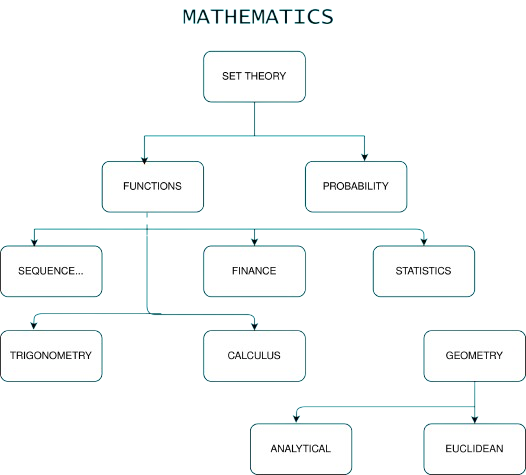
\includegraphics[keepaspectratio]{images/Structure.png}}\hfill

in the order of seen from the table of contents. I've structured the
book such that one chapter builds from the previous one. To master
Probability and Functions, it would be helpful if you did Set Theory
first --- although not neccessary(\textbf{RECOMMENDED}). The rest can be
seen from the Mind-map intuitively so.

\subsubsection*{NOTE :}\label{note}
\addcontentsline{toc}{subsubsection}{NOTE :}

This is an on-going project. The resources used will be cited. Slowly
but surely, step by step. \textbf{Enjoy!}

\bookmarksetup{startatroot}

\chapter{Set Theory: An Introduction}\label{set-theory-an-introduction}

\section{History}\label{history}

The idea of grouping things has existed for the longest of time in the
history of the Modern Homo Sapiens specie. The study of grouping objects
was later called set theory, where a \textbf{set} is a
collection/grouping of objects. The study of modern set theory is often
attributed to one of its founders, a prominent German
mathematician---George Cantor along with another German mathematician
Richard Dedekind, which they developed in the 1870s.

\begin{figure}[H]

{\centering \pandocbounded{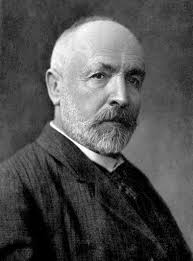
\includegraphics[keepaspectratio]{images/G.Cantor.jpeg}}

}

\caption{George Cantor}

\end{figure}%

As the topic was relatively new and hot at the time, it received
backlashes often from older mathematicians who did not embrace new idea.
A famous mathematician and philosopher, Bertrand Russell also attacked
some of these ideas which gave birth to a concepts like Russell's
Paradoxes or fuzzy set theory.

\section{Applications}\label{applications}

\textbf{Yatla \textbar{} UNDER CONSTRUCTION}

However, as I've outline that this isn't a new idea, you have also used
sets in your daily life. Formally, a

\begin{description}
\item[SET]
is a collection of objects or elements. A set is often denoted with a
capital letter \& curly braces.
\end{description}

These objects are also called members. A classroom is a set made of
students, and these students are the members of this set. In that same
classroom, we can have a set which consists of only boys. Remember that
the art of grouping can group things that have similarities or are
entirely different. The classroom set has both girls and boys. The
similarity is that they're all human. The set grouping all boys in that
classroom share the similarity being that they're boys, but they're most
likely different in many other ways, from names to their Blood Pressure.
A set is often denoted with a capital letter \& curly braces , while the
elements are denoted by small letters .Let \[
V = \{𝑎,𝑒,𝑖,𝑜,𝑢\}
\] Be an example where the set \(V\) is the set of all vowels. Where
\(𝑎,𝑒,𝑖,𝑜,𝑢\) are the members of the set \(V\). The curly braces means
``the set of''. Since \(u\) and \(a, 𝑒,𝑖, 𝑜,𝑢\) are elements of \(V\),
we denote it as \(u𝜖V\) and \[(𝑎,𝑒,𝑖,𝑜,𝑢)𝜖V ≡ 𝑎,𝑒,𝑖,𝑜,𝑢𝜖V\]

Respectively. It oath to be noted that the \emph{order} of elements in
the set and \emph{repetition} are not important, thus a set with
elements \[\{𝑜, 𝑒, 𝑢,𝑎,𝑖\}\] and \[\{𝑎,𝑎,𝑖,𝑖,𝑖,𝑖,𝑖,𝑜,𝑢,𝑒,𝑒\} \] Are the
same as the set \(V\). The number of elements within a set are referred
to as a \textbf{Cardinality}, denoted by the absolute bars \(|𝑋|\) where
\(X\) is a set. Thus the cardinality of the set of vowels \(𝑉\) is \(5\)
denoted \[|V| = 5\].

Another simple example would be as follows, lets call it the
\textbf{\emph{Black Box example}} :

Suppose you have a Black Box in a class, then ask each and every student
to put a paper inside of the box(more like voting). The papers could be
different colors and shapes, or just all plain White square papers.\\
The Box will act as a set while the papers of the students inside the
box are regarded as the elements of the set(or elements of the box). If
the box was empty, then we'd say the box is an \textbf{empty set/null
set}. This is a special case of a set and it is denoted by

\(\phi\) or empty curly braces \(\{\}\). In turn, \(\phi = \{\}\) with a
cardinality of \(0\).

\section{Example}\label{example}

Suppose there are three sets \[A = \phi \] \[B = \{\phi\} \]
\[C = \{\} \]

\begin{enumerate}
\def\labelenumi{\arabic{enumi}.}
\tightlist
\item
  Which of these are equal?

  \begin{enumerate}
  \def\labelenumii{\alph{enumii}.}
  \tightlist
  \item
    𝐴 and 𝐵
  \item
    𝐴 and 𝐶
  \item
    𝐵 and 𝐶
  \end{enumerate}
\item
  What are the cardinalities of each set?
\end{enumerate}

\subsection{Solution}\label{solution}

\textbf{UNDER CONSTRUCTION}

\bookmarksetup{startatroot}

\chapter{Probability}\label{probability}

\textbf{UNDER CONSTRUCTION}

\bookmarksetup{startatroot}

\chapter{Combinorics : Counting
Principles}\label{combinorics-counting-principles}

\bookmarksetup{startatroot}

\chapter{Functions}\label{functions}

\bookmarksetup{startatroot}

\chapter*{Polynomials}\label{polynomials}
\addcontentsline{toc}{chapter}{Polynomials}

\markboth{Polynomials}{Polynomials}

\bookmarksetup{startatroot}

\chapter*{Trigonometry}\label{trigonometry}
\addcontentsline{toc}{chapter}{Trigonometry}

\markboth{Trigonometry}{Trigonometry}

\textbf{UNDER CONSTRUCTION}

\bookmarksetup{startatroot}

\chapter{Sequence \& Series}\label{sequence-series}

\section{History}\label{history-1}

The idea of sequences and series' go a long way back into the past. One
of the earliest encounters could be seen around 5th BCE where the famous
Greek philosopher \emph{Zeno of Elea} introduced a number of problems
where only Nine survived, which came to be known as Zeno's Paradoxes,
these were his proposals to the questions concerning space and time at
their time.

\begin{figure}[H]

{\centering \pandocbounded{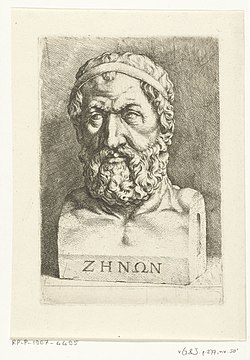
\includegraphics[keepaspectratio]{images/ZenoVanElea.jpg}}

}

\caption{Zeno of Elea}

\end{figure}%

On one of them, Zeno argued that a man who wanted to walk across a room,
had to walk half the distance of the room first, but before travelling
that distance they had to travel halfway of that half, then half of
that, and repeatedly infinitely many times producing the sequence \[
...,\frac{1}{16},\frac{1}{8},\frac{1}{4},\frac{1}{2},1
\]

Which he claimed was impossible since it requires a number of infinite
tasks and wouldn't have the first distance to travel, meaning the
journey wouldn't even start. Traveling across the same room would give
the sequence \[
1,\frac{1}{2},\frac{1}{4},\frac{1}{8},\frac{1}{16},...,\frac{1}{2^n}
\]

\section{Applications}\label{applications-1}

This sequence is popularly known as the Geometric sequence. More about
that later. In present day, sequence and series has become increasingly
important as it is widely used in almost every field. In finance it is
used to calculate the return of loans and investments, in physics it is
used to study waves and their properties. In Chemistry it is used to see
how chemical reactions end, in Statistics it is used to study trends, in
ecology and epidemiology it is used to model populations of the same and
different species. In astronomy and cosmology it is used to study the
emission of radiation/energy of celestial bodies; and it is used by
TikTok and Netflix to recommend you videos and movies you may like.\\
First and foremost, what's the difference between a sequence and a
series?

\section{Introduction}\label{introduction}

\begin{description}
\item[SEQUENCE]
a list of ordered numbers separated by a comma
\end{description}

e.g.~\[1,2,3,4,…,𝑛\] where \(1\) is the 1st term denoted by \(T_1\)
\[2,4,6,8,…,2n\] where \(2n\) is the formula for the sequence denoted
\(𝑇_𝑛\) \[3,6,9,12,…,2𝑛+1\]

Thus, a sequence is denoted by \[
1, 𝑇_2, 𝑇_3,…,𝑇_𝑛 
\]

\begin{description}
\item[SERIES]
the sum of individual terms that form a sequence, separated by an
operator \(\pm\)
\end{description}

e.g.~\[1 + 2 +3+4+⋯ \] \[2 +4+6+8+⋯ \] \[3 +6+9+12+⋯ \] Thus, a series
is denoted by \[
S_n = 𝑇_1 +𝑇_2+𝑇_3+⋯+𝑇_𝑛 = \sum_{i=1}^{n}T_i
\] Where \[
 S_1 = 𝑇_1 
\] \[
 𝑆_2 = 𝑇_1 +T_2 = \sum_{i=1}^{2} T_𝑖
\] \[
 𝑆_3 = 𝑇_1 +T_2 +T_3 = \sum_{i=1}^{3} T_𝑖
\] There are recursive and non-recursive sequences.

\begin{description}
\item[RECURSIVE]
these are sequences which whose terms are dependent on the previous
term. They are a `regress'.
\end{description}

A very famous one is the Fibonacci sequence that appears a lot in
nature, especially in the rows of corn or becomes the sequence of the
petals on a flower. \emph{Fibonacci sequence} : \[0,1,1,2,3,5,8,13,… \]
Another interesting example is the logistic equation, which is often a
realistic approach used to model the population of species.

\begin{description}
\item[NON-RECURSIVE]
sequences that are not recursive. These are the `normal' ones.
\end{description}

We'll only be dealing with the Arithmetic(linear), Quadratic and
Geometric sequences and series'.

\section*{Arithmetic}\label{arithmetic}
\addcontentsline{toc}{section}{Arithmetic}

\markright{Arithmetic}

\subsection{Arithmetic Sequence}\label{arithmetic-sequence}

An Arithmetic sequence can be seen as a linear function where the \(c\)
in \[y = mx+c \] can either be negative or positive. This is a
constant(fixed) number that is added to each previous term to find the
next. For the sake of formality, in this chapter we use the notation \[
T_n = 𝜙𝑛+𝛾                         
\]

But more importantly, to obtain the equation in 2.2 , we use the
equation \[
T_n= 𝑎+(𝑛−1)𝑑                               
\] Where \(𝜙 = d\) and \$𝛾 = 𝑎−𝑑 \$. Here \(𝑇_𝑛\) denotes the general
term, 𝑎 the first term of the sequence and 𝑑 is the common difference.
Since a sequence is defined by

\[
T_1,T_2,T_3,...,T_n
\]

\subsection{Arithmetic Series}\label{arithmetic-series}

\section*{Geometric}\label{geometric}
\addcontentsline{toc}{section}{Geometric}

\markright{Geometric}

\subsection{Geometric Sequence}\label{geometric-sequence}

\subsection{Geometric Series}\label{geometric-series}

\subsubsection{Infinite Geometric
Series}\label{infinite-geometric-series}

\textbf{UNDER CONSTRUCTION}

\bookmarksetup{startatroot}

\chapter{Financancial Mathematics}\label{financancial-mathematics}

\textbf{UNDER CONSTRUCTION}

\bookmarksetup{startatroot}

\chapter{Calculus}\label{calculus}

\textbf{UNDER CONSTRUCTION}

\bookmarksetup{startatroot}

\chapter{Statistics}\label{statistics}

\textbf{UNDER CONSTRUCTION}

\bookmarksetup{startatroot}

\chapter{Geometry}\label{geometry}

\bookmarksetup{startatroot}

\chapter*{Analytical Geometry}\label{analytical-geometry}
\addcontentsline{toc}{chapter}{Analytical Geometry}

\markboth{Analytical Geometry}{Analytical Geometry}

\textbf{UNDER CONSTRUCTION}

\bookmarksetup{startatroot}

\chapter*{Euclidean Geometry}\label{euclidean-geometry}
\addcontentsline{toc}{chapter}{Euclidean Geometry}

\markboth{Euclidean Geometry}{Euclidean Geometry}

\bookmarksetup{startatroot}

\chapter*{References}\label{references}
\addcontentsline{toc}{chapter}{References}

\markboth{References}{References}

\phantomsection\label{refs}
\begin{CSLReferences}{0}{1}
\end{CSLReferences}




\end{document}
